\section{Generación de código y verificación de software}

\subsection{Implementación del controlador}

El controlador se separó de la planta en su propio modelo, \texttt{Controller\_BoP.slx}, que es
el sistema bajo prueba de las etapas siguientes y se conserva como referencia sin cambios. El
modelo es de un solo eje: el firmware lo instancia dos veces. Tiene cuatro entradas, la
referencia $r$ en \si{\milli\metre}, la posición filtrada $\xh$ en \si{\milli\metre}, la velocidad
$\vh$ en \si{\milli\metre\per\second} y la señal lógica \texttt{habilitado}, y tres salidas: la
inclinación pedida $\thc$ en \si{\radian}, el estado del integrador $I$ en \si{\radian} y la
bandera \texttt{saturado}. Con \texttt{habilitado} en falso, que corresponde al arranque, a la
pérdida de la bola o al disparo del watchdog, la salida es cero y el integrador se reinicia. El
modelo corre a $\Ts = \SI{33.3}{\milli\second}\ (\SI{30}{\hertz})$ y la ley \eqref{eq:ley} se escribió en una sola función
de MATLAB que usan tanto el MIL como el bloque del modelo, de modo que hay una sola fuente del
algoritmo. En la Fig.~\ref{fig:controller} se ven las cuatro entradas de la interfaz, los ocho
parámetros como bloques \texttt{Constant} y un solo bloque con la ley; la planta no está.

\begin{figure}[!t]
\centering
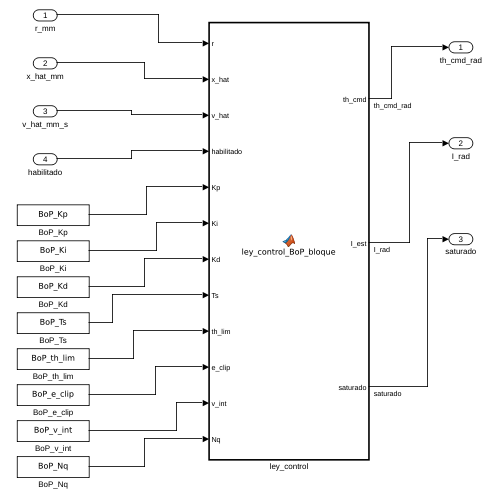
\includegraphics[width=0.85\columnwidth]{figuras/Controller_BoP_slx.png}
\caption{Modelo \texttt{Controller\_BoP.slx} (vista generada por Simulink): las cuatro entradas
de la interfaz, los ocho parámetros calibrables como bloques \texttt{Constant} y el bloque
\texttt{ley\_control}, que implementa \eqref{eq:ley}.}
\label{fig:controller}
\end{figure}

De la configuración de generación de código solo importan cuatro puntos para entender la
implementación. Se usó el destino \texttt{ert.tlc} de Embedded Coder con interfaz
\emph{Reusable function}, para que el estado viaje en una estructura y cada eje tenga la suya
\cite{mw_codegen}. Los datos son \texttt{double}. Los ocho parámetros del controlador son
\texttt{Simulink.Parameter} con clase de almacenamiento \texttt{ExportedGlobal}, así que quedan
como variables globales calibrables. Y el hardware se configuró como un procesador genérico de
\SI{32}{bits} \emph{little-endian}, con división entera que redondea hacia cero, que es lo que
permitió compilar el mismo código en la PC (SIL) y en la ESP32 (PIL). El Code Generation Advisor
dio \num{0} resultados Fail, \num{5} advertencias y \num{26} verificaciones aprobadas; las
advertencias se revisaron y justificaron una por una, sin usar correcciones automáticas.

Las cinco advertencias fueron: los objetivos de generación del Advisor no coincidían con los
fijados en el modelo (eficiencia y trazabilidad), lo que es informativo; el diagnóstico de nombres
duplicados de \emph{Data Store} no está en error, y el modelo no usa \emph{Data Stores}; el orden
de bytes y el redondeo de la división entera no estaban definidos, lo que se corrigió con la
configuración de hardware descrita arriba; el código admite números no finitos, que hacen falta
porque la función \texttt{sign} de MATLAB maneja \texttt{NaN}; y hay comparaciones de igualdad
entre valores en punto flotante, que son intencionales, porque \texttt{saturado} se define
como $\thc \ne u$.

\subsection{Inspección del código generado}

Antes de generar código se comprobó que el modelo reproduce el MIL: en cinco ensayos, incluido
uno con saturación, la diferencia entre el modelo y la ley usada en el MIL fue exactamente cero
en $\thc$, $I$ y \texttt{saturado}. Después se inspeccionó el código generado. La
Tabla~\ref{tab:codigo} resume la correspondencia.

\begin{table}[!t]
\caption{Correspondencia entre el modelo y el código generado (\texttt{Controller\_BoP.c} y
\texttt{.h}). Fuente: \texttt{etapaE/tabla\_modelo\_codigo.md}.}
\label{tab:codigo}
\centering
\footnotesize
\setlength{\tabcolsep}{3pt}
\begin{tabular}{@{}p{0.30\columnwidth}p{0.62\columnwidth}@{}}
\toprule
\textbf{Característica} & \textbf{Evidencia en el código} \\
\midrule
Interfaz & \texttt{Controller\_BoP\_step(M, r, x\_hat, v\_hat, hab, \&th, \&I, \&sat)}, tipos \texttt{real\_T} y \texttt{boolean\_T} \\
Estado interno & \texttt{DW\_Controller\_BoP\_T.I} y \texttt{.nq}, uno por instancia \\
Parámetros calibrables & \texttt{BoP\_Kp}, \texttt{BoP\_Ki}, \texttt{BoP\_Kd}, \texttt{BoP\_Ts}, \texttt{BoP\_th\_lim}, \texttt{BoP\_e\_clip}, \texttt{BoP\_v\_int}, \texttt{BoP\_Nq} como globales \\
Saturación & \texttt{fmin(fmax(u, -BoP\_th\_lim), BoP\_th\_lim)} \\
Integración condicional & \texttt{if (fabs(v\_hat) < BoP\_v\_int) nq++; else nq = 0;} \\
Anti-windup & El integrador no avanza si está saturado y $\operatorname{sign}(\varepsilon) = \operatorname{sign}(u)$ \\
Planta & Ausente: el código solo contiene la ley de control \\
\bottomrule
\end{tabular}
\end{table}

\begin{lstlisting}
a__1 = (BoP_Kp*eps_ + DW->I) + BoP_Kd*v_hat;
*th_cmd = fmin(fmax(a__1, -BoP_th_lim), BoP_th_lim);
\end{lstlisting}

El fragmento conserva el mismo orden de operaciones que el modelo. El código compilado con
\texttt{gcc} en la PC reprodujo el MIL con una diferencia máxima de \SI{4e-11}{\radian}, que
corresponde al redondeo de los CSV usados como referencia.

\subsection{Verificación Software-in-the-Loop}

El banco \texttt{BoP\_Test\_SIL.slx} tiene dos ramas en la misma simulación, Normal y SIL
\cite{mw_sil}. Comparten la referencia (cero y, a los \SI{4.5}{\second}, \SI{50}{\milli\metre} en
cada eje), la habilitación desde \SI{0.5}{\second}, la condición inicial de la bola en
$(80, -60)\,\si{\milli\metre}$, $\Ts$, la secuencia de ruido y el tiempo de \SI{9}{\second}. Cada
rama tiene su propia planta no lineal de dos ejes y sus dos instancias del controlador, porque
las acciones de control se calculan por separado. La Fig.~\ref{fig:sil} muestra la diferencia
$\Delta\theta_x = \theta_{x,\mathrm{SIL}} - \theta_{x,\mathrm{Normal}}$ y
$\Delta x = x_{\mathrm{SIL}} - x_{\mathrm{Normal}}$ junto con la trayectoria.

\begin{figure}[!t]
\centering
\begin{tikzpicture}
\begin{groupplot}[group style={group size=1 by 2, vertical sep=0.7cm}, estilo, height=3.2cm,
                  xmin=0, xmax=9]
\nextgroupplot[ylabel={Posición (\si{\milli\metre})}, xticklabels={}, legend pos=south east,
               legend columns=2]
  \addplot[cAzul] table[col sep=comma, x=t_s, y=Normal_x] {\G/F1_comparacion.csv};
  \addplot[cNaranja, dashed] table[col sep=comma, x=t_s, y=Normal_y] {\G/F1_comparacion.csv};
  \legend{$x$, $y$}
\nextgroupplot[ylabel={Diferencia}, xlabel={Tiempo (\si{\second})}, ymin=-1, ymax=1,
               legend pos=north east, legend columns=2]
  \addplot[cRojo] table[col sep=comma, x=t_s, y=dif_thx] {\G/F1_comparacion.csv};
  \addplot[cVerde, dashed] table[col sep=comma, x=t_s, y=dif_x] {\G/F1_comparacion.csv};
  \addplot[cNaranja, densely dotted, line width=1.1pt] table[col sep=comma, x=t_s, y=dif_thx] {\G/G5_comparacion.csv};
  \addplot[cAzul, dashdotted] table[col sep=comma, x=t_s, y=dif_x] {\G/G5_comparacion.csv};
  \legend{SIL $\Delta\theta_x$ (\si{\radian}), SIL $\Delta x$ (\si{\milli\metre}), PIL $\Delta\theta_x$, PIL $\Delta x$}
\end{groupplot}
\end{tikzpicture}
\caption{Bancos SIL y PIL. Arriba: trayectoria de la rama Normal. Abajo: diferencias
SIL $-$ Normal y PIL $-$ Normal (G5), idénticamente nulas en las \num{271} muestras.}
\label{fig:sil}
\end{figure}

En las \num{271} muestras y en las diez señales comparadas ($\thc$, $I$ y \texttt{saturado} de
cada eje, y $\xh$, $x$, $y$ de la planta) la diferencia máxima y el RMSE fueron cero, con igualdad
exacta (Tabla~\ref{tab:silpil}). La prueba satisface el criterio de equivalencia. SIL verifica
que el código generado, compilado en la PC, calcula lo mismo que el modelo dentro del lazo
cerrado. No verifica que funcione en la ESP32, ni con su compilador y su aritmética, ni con la
planta real. Además, este ensayo no lleva el controlador a la saturación; esa rama del código se
comprobó en la equivalencia previa y vuelve a probarse en PIL.
